\documentclass[../../../analisi-dei-requisiti.tex]{subfiles}

\begin{document}

\subsubsection{AUC11: Eliminazione gestore}%
\label{subs:AUC11}

\begin{figure}[H]
  \centering
  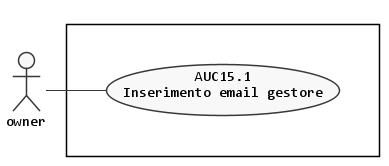
\includegraphics[width=100mm]{eliminazione-gestore.png}
  \caption{AUC11: Eliminazione gestore}%
  \label{fig:AUC11}
\end{figure}

\begin{description}
  \item[Codice:] AUC11;
  \item[Titolo:] Eliminazione gestore;
  \item[Attori primari:] owner;
  \item[Precondizione:] il sistema deve rendere disponibile la pagina di eliminazione gestore;
  \item[Postcondizione:] l'utente non è più gestore;
  \item[Scenario principale:]
  \begin{enumerate}
    \item l'owner vuole eliminare i privilegi ad un utente gestore.
  \end{enumerate}
\end{description}

\subsubsection{AUC11.1: Inserimento email gestore}%
\label{subs:AUC11.1}
\begin{description}
  \item[Codice:] AUC11.1;
  \item[Titolo:] Inserimento email gestore;
  \item[Attori primari:] owner;
  \item[Precondizione:] il sistema deve rendere disponibile la possibilità di inserire l'email del gestore da eliminare;
  \item[Postcondizione:] l'email viene opportunemente inserita;
  \item[Scenario principale:]
  \begin{enumerate}
    \item l'owner inserisce l'email del gestore da eliminare.
  \end{enumerate}
\end{description}

\end{document}
